\documentclass[11pt,letterpaper]{article}
\usepackage[lmargin=1in,rmargin=1in,tmargin=1in,bmargin=1in]{geometry}
\usepackage{../style/homework}
\usepackage{../style/commands}
\setbool{quotetype}{true} % True: Side; False: Under
\setbool{hideans}{false} % Student: True; Instructor: False

% -------------------
% Content
% -------------------
\begin{document}

\homework{6: Due 11/04}{I used to sell furniture for a living. The trouble was, it was my own.}{Les Dawson}

% Problem 1
\problem{10} As accurately as possible, sketch the feasible region given by the following maximization problem:
	\[
	\begin{aligned}
	\text{max } z= &\;4x_1 + 6x_2 \\
	x_1 + x_2&\leq 10 \\
	2x_1 - x_2&\geq 2 \\
	x_1, x_2&\geq 0
	\end{aligned}
	\]
Is this region bounded or unbounded? \pspace

\sol The first inequality corresponds to the inequality $x + y \leq 10$. Solving for $y$, we have $y \leq 10 - x$. So we plot the line $y= 10 - x$. On this line, $y= 10 - x$ and because we want $y \leq 10 - x$, we shade below the line. The second equality corresponds to the inequality $2x - y \geq 2$. Solving for $y$, we have $2x - 2 \geq y$, i.e. $y \leq 2x - 2$. So we plot the line $y= 2x - 2$. On this line, $y= 2x - 2$ and because we want $y \leq 2x - 2$, we shade beneath the line. The final inequalities correspond to the inequalities $x, y \geq 0$. This means we only consider things in Quadrant~I. Plotting all these conditions, we obtain the feasible reason shaded below. 
	\[
	\fbox{
	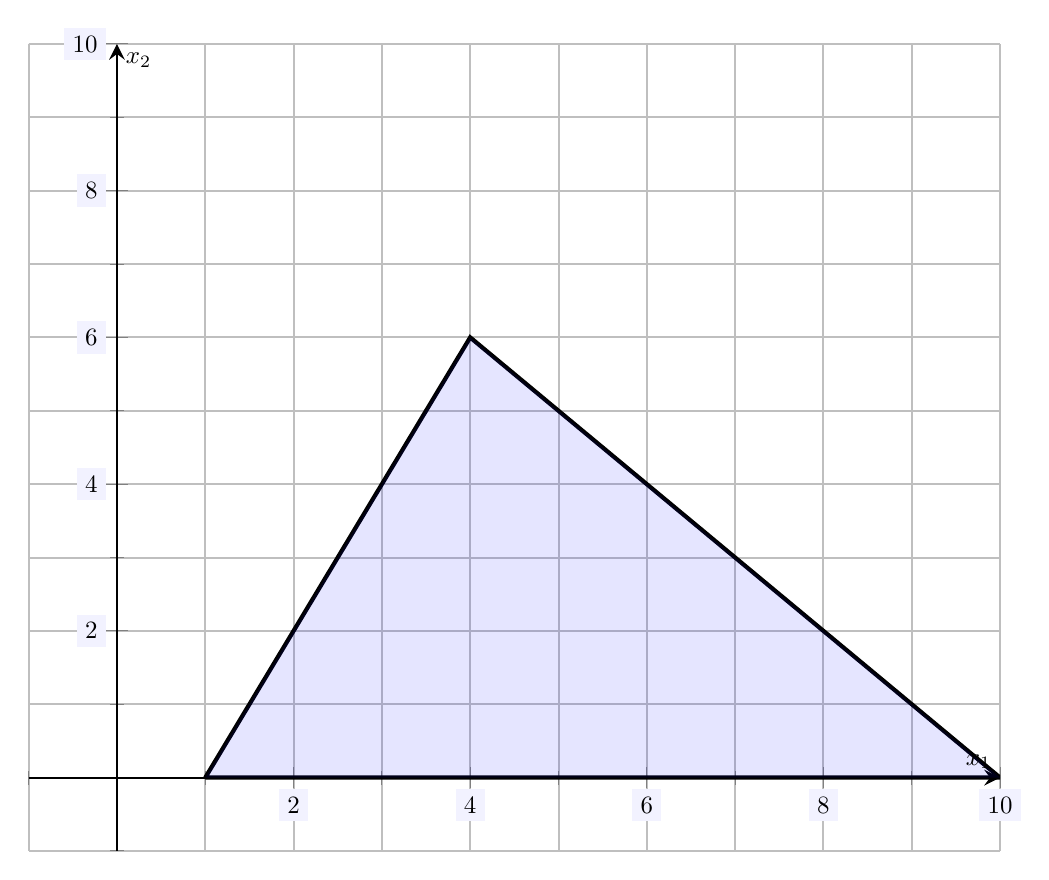
\begin{tikzpicture}[scale=1.8,every node/.style={scale=0.5}]
	\begin{axis}[
	grid=both,
	axis lines=middle,
	ticklabel style={fill=blue!5!white},
	xmin= -1, xmax=10,
	ymin= -1, ymax=10,
	xtick={0,2,4,6,8,10},
	ytick={0,2,4,6,8,10},
	minor tick = {-1,0,1,...,10},
	xlabel=\(x_1\),ylabel=\(x_2\),
	]
	\draw[line width=0.03cm] (1,0) -- (4,6) -- (10,0) -- (1,0);
	\draw[line width=0.01cm,fill= blue,opacity=0.1] (1,0) -- (4,6) -- (10,0) -- (1,0);
	\end{axis}
	\end{tikzpicture}
	}
	\]
Clearly, this region is bounded. 





\newpage





% Problem 2
\problem{10} As accurately as possible, sketch the feasible region given by the following minimization problem:
	\[
	\begin{aligned}
	\text{min } z= &\;x_1 - 3x_2 \\
	x_1 + x_2&\geq 4 \\
	\frac{1}{2}\,x_1 + 3x_2&\geq 7 \\
	x_1, x_2&\geq 0
	\end{aligned}
	\]
Is this region bounded or unbounded? \pspace

\sol The first inequality correspond to the inequality $x + y \geq 4$. Solving for $y$, we find $y \geq 4 - x$. So we plot the line $y= 4 - x$. On the line, $y= 4 - x$ and because we want $y \geq 4 - x$, we shade above the line. The second equality corresponds to the inequality $\frac{1}{2}\,x + 3y \geq 7$. Solving for $y$, we find $y \geq -\frac{1}{6}x + \frac{7}{3}= \frac{14 - x}{6}$. On the line, $y= -\frac{1}{6}x + \frac{7}{3}$ and because we want $y \geq -\frac{1}{6}x + \frac{7}{3}$, we shade above the line. The final inequalities correspond to the inequalities $x, y \geq 0$. This means we only consider things in Quadrant~I. Plotting all these conditions, we obtain the feasible reason shaded below. 
	\[
	\fbox{
	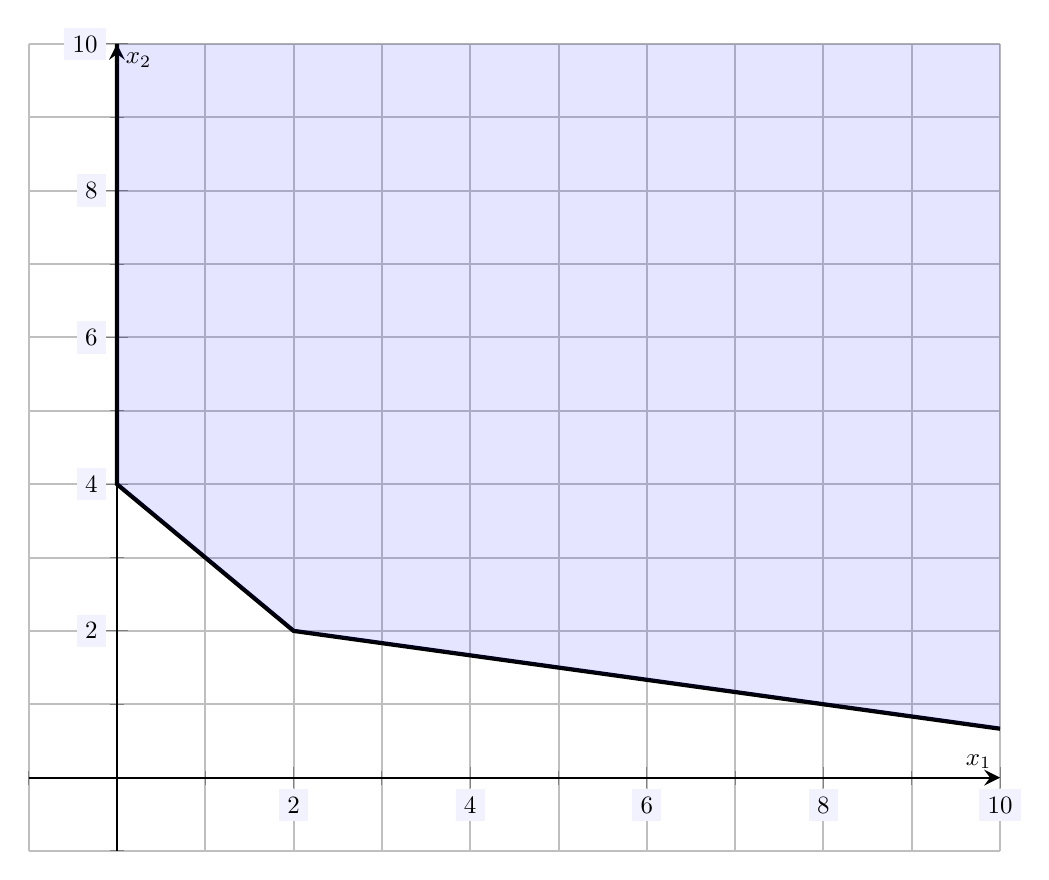
\begin{tikzpicture}[scale=1.8,every node/.style={scale=0.5}]
	\begin{axis}[
	grid=both,
	axis lines=middle,
	ticklabel style={fill=blue!5!white},
	xmin= -1, xmax=10,
	ymin= -1, ymax=10,
	xtick={0,2,4,6,8,10},
	ytick={0,2,4,6,8,10},
	minor tick = {-1,0,1,...,10},
	xlabel=\(x_1\),ylabel=\(x_2\),
	]
	\draw[line width=0.03cm] (10,2/3) -- (2,2) -- (0,4) -- (0,10);
	\draw[line width=0.01cm,fill= blue,opacity=0.1] (10,2/3) -- (2,2) -- (0,4) -- (0,10) -- (10,10) -- (10,2/3);
	\end{axis}
	\end{tikzpicture}
	}
	\]
Clearly, this region is unbounded.





\newpage





% Problem 3
\problem{10} Find a system of inequalities that gives the following feasible region:
	\[
	\fbox{
	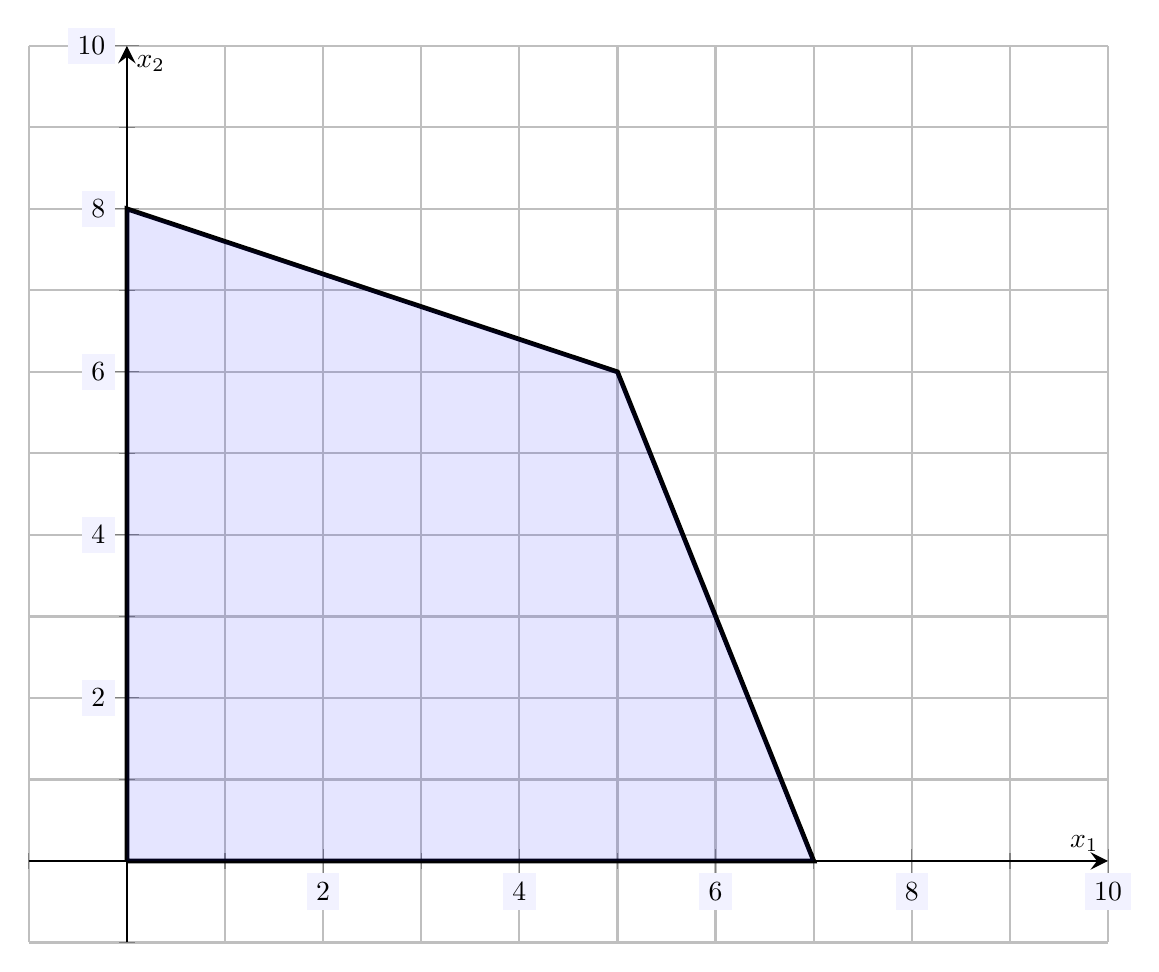
\begin{tikzpicture}[scale=2,every node/.style={scale=0.5}]
	\begin{axis}[
	grid=both,
	axis lines=middle,
	ticklabel style={fill=blue!5!white},
	xmin= -1, xmax=10,
	ymin= -1, ymax=10,
	xtick={0,2,4,6,8,10},
	ytick={0,2,4,6,8,10},
	minor tick = {-1,0,1,...,10},
	xlabel=\(x_1\),ylabel=\(x_2\),
	]
	\draw[line width=0.03cm] (0,0) -- (0,8) -- (5,6) -- (7,0) -- (0,0);
	\draw[line width=0.01cm,fill= blue,opacity=0.1] (0,0) -- (0,8) -- (5,6) -- (7,0) -- (0,0);
	\end{axis}
	\end{tikzpicture}
	}
	\] \pspace

\sol To force us to be in Quadrant~I, we can use the inequalities $x_1, x_2 \geq 0$. Now we find the equations of the two lines, the `uppermost' containing the points $(0,8)$ and $(5,6)$ and the `rightmost' containing the points $(5,6)$ and $(7,0)$. In the former case, the line is $y= -\frac{2}{5}x + 8$, and in the latter case, $y= -3x + 21$. Because we want to shade below these lines, we have $y \leq -\frac{2}{5}x + 8$, i.e. $\frac{2}{5}x + y \leq 8$, and $y \leq -3x + 21$, i.e. $3x + y \leq 21$. Therefore, a system of inequalities (using $x_1= x$ and $x_2= y$) representing this feasible region is\dots
	\[
	\begin{aligned}
	\frac{2}{5}\,x_1 + x_2&\leq 8 \\
	3x_1 + x_2&\leq 21 \\
	x_1, x_2&\geq 0
	\end{aligned}
	\]





\newpage





% Problem 4
\problem{10} Use the Fundamental Theorem of Linear Programming, i.e. the Corner-Point Method, to find the maximum and minimum values for $z$ given the following definition of $z$ and constraints:
	\[
	\begin{aligned}
	z= -2x_1 &+ 5x_2 \\
	-x_1 + x_2&\leq 4 \\
	4x_1 + x_2&\leq 24 \\
	x_1, x_2 &\geq 0
	\end{aligned}
	\]
	\[
	\fbox{
	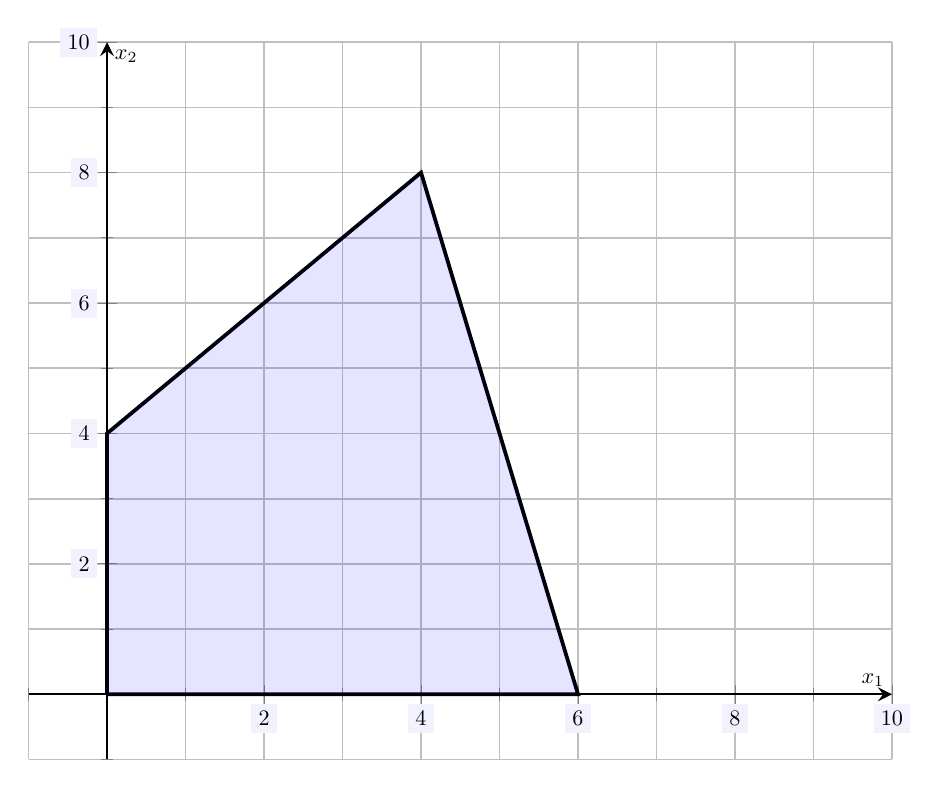
\begin{tikzpicture}[scale=1.6,every node/.style={scale=0.5}]
	\begin{axis}[
	grid=both,
	axis lines=middle,
	ticklabel style={fill=blue!5!white},
	xmin= -1, xmax=10,
	ymin= -1, ymax=10,
	xtick={0,2,4,6,8,10},
	ytick={0,2,4,6,8,10},
	minor tick = {-1,0,1,...,10},
	xlabel=\(x_1\),ylabel=\(x_2\),
	]
	\draw[line width=0.03cm] (0,0) -- (0,4) -- (4,8) -- (6,0) -- (0,0);
	\draw[line width=0.01cm,fill= blue,opacity=0.1] (0,0) -- (0,4) -- (4,8) -- (6,0) -- (0,0);
	\end{axis}
	\end{tikzpicture}
	}
	\]

\sol The Fundamental Theorem of Linear Programming says that if we have a linear programming problem, i.e. a maximization or minimization of a linear function, over a nonempty bounded region, then the maximum and minimum exist and occur at a corner point. So we plot our feasible region, check that it is nonempty and bounded, find the corner points, and evaluate $z$ at these points. The first inequality corresponds to the line $y= x + 4$, shaded below. The second inequality corresponds to the line $y= 24 - 4x$, shaded below. The last inequalities simply imply that we are in Quadrant~I. We then plot these lines. We find the line $y= x + 4$ has $x$-intercept $(-4, 0)$, $y$-intercept $(0, 4)$, and intersects the line $y= 24 - 4x$ at the point $(4,8)$. The line $y= 24 - 4x$ has $x$-intercept $(6, 0)$ and $y$-intercept $(0, 24)$. Therefore, the corner points for this feasible region (notice the region is bounded) are $(0, 0)$, $(0, 4)$, $(4, 8)$, and $(6, 0)$. We evaluate $z= -2x_1 + 5x_2= -2x + 5y$ at these points:
	\begin{table}[!ht]
	\centering
	\begin{tabular}{l|l}
	$(x, y)$ & $z= -2x + 5y$ \\ \hline
	$(0, 0)$ & $z= 0 + 0= 0$ \\
	$(0, 4)$ & $z= 0 + 20= 20$ \\
	$(4, 8)$ & $z= -8 + 40= 32$ \\
	$(6, 0)$ & $z= -12 + 0= -12$
	\end{tabular}
	\end{table} \par	
Therefore, the minimum value for $z$ is $-12$ and occurs at $(x_1, x_2)= (6, 0)$, and the maximum value for $z$ is $32$ and occurs at $(x_1, x_2)= (4, 8)$. 


\end{document}